\section{Source Evidence for the Skill Bottleneck}
\label{sec:evidence}
TimeSage-EV evaluates recurring analysis over institutional releases from February 2023 through May 2026 \citep{yao2026timesage}. The benchmark reports persistent gaps in temporal validity. It also reports recurring difficulty with exogenous context. These failures remain visible across model tiers, which makes them suitable targets for reusable procedure induction.

The source paper introduces TimeSage-1.0 as a diagnostic self-evolving harness. The base interface remains aligned with the baseline. The skill-library manager is the additional mechanism. Skills are induced from previous reasoning traces and become available to later periods. This gives the benchmark an explicit state-update boundary for testing reusable procedures.

The released aggregate results support the value of this state. Reusable skills improve overall performance, with the clearest gains on medium and hard scenarios. Skill invocation is most frequent on hard scenarios. The source also reports that the skill-enabled condition reduces token cost to 0.82$\times$ the reference condition.

\begin{figure}[t]
\centering
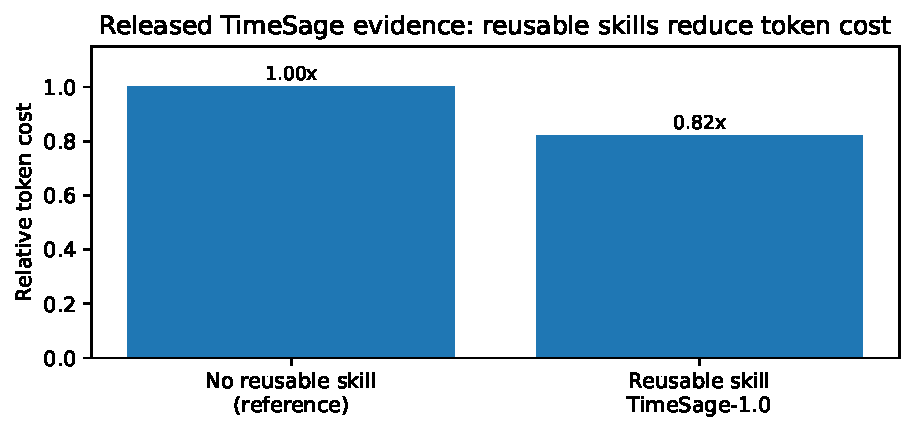
\includegraphics[width=0.9\linewidth]{figures/fig2_source_skill_efficiency.pdf}
\caption{Released TimeSage evidence reports 0.82$\times$ relative token cost when reusable skills are enabled. The source also reports higher benchmark performance under the skill-library condition.}
\label{fig:source}
\end{figure}

These results establish three ingredients for the causal hypothesis. Reusable procedures can enter persistent state. They can influence later periods. They improve aggregate performance while reducing repeated reasoning cost. The remaining question concerns mechanism specificity: which recurring failure families are repaired by which skill?

The benchmark Appendix provides the needed intervention surface. \texttt{induct\_skill} stores a reusable function with a description and notes. \texttt{retrieve\_skill} exposes the stored implementation when the short description is insufficient. Skills accepted after period $t$ become callable from period $t+1$. This chronological registration preserves the evolving evaluation structure.

The source also gives examples of desirable skill granularity. It encourages compact procedures such as schema-specific loaders and date-to-period converters. Scenario-specific answer dictionaries are discouraged. This contract aligns directly with our targeted temporal-skill design.
